\chapter{Introduction}
\label{chap:intro}

%%%%%%%%%%%%%%%%%%%%%%%%%%%%%%%%%%%%%%%%%%%%%%%%%%%%%%%%%%%%%%%%%%%%%%%%%%%%%%%
\section{Motivation}
\label{sec:chap1-motivation}

%Intro paragraph\\
%-talk about the increasingly important role of simulation in nuclear?\\
%-challenges for today's nuclear fleet which simulation is well-poised to tackle\\
%-segue into talk about nuclear reactor / neutron physics paragraph\\
%-based on empirical models\\
%-need to account for angular dependence of neutron flux (e.g. "transport" methods)\\

Numerical simulation has long played an important role in nuclear reactor physics and engineering. The nuclear industry relies on computational modeling of the neutron physics in reactors to predict core reactivity, power distributions, fuel depletion, and transient behavior to ensure the safety and reliability of the current fleet of Light Water Reactors (LWRs). Predictive simulations are necessary to evaluate innovations which seek to improve reactor safety and fuel cycle economics, such as reduced safety margins, accident-tolerant fuels, and extended cycle lengths. In addition, simulation is used to assess the technical competencies of advanced reactor technologies such as Small Modular Reactors (SMRs), Sodium Fast Reactors (SFRs), Molten Salt Reactors (MSRs), High Temperature Gas Reactors (HTGRs), among other proposed designs. 

Many Generation III+ reactors, such as the Westinghouse AP1000\texttrademark \ac{PWR}, optimize performance with complicated core designs. A variety of reactivity control mechanisms -- including partially-inserted control rods, ``grey'' control poisons, Integral Fuel Burnable Absorbers (IFBA), soluble boron, etc. -- along with axial enrichment zoning are used to improve performance metrics such as power peaking factors. The reactor analysis methods in widespread use today assume a ``smoothly'' varying flux distribution, and are not well-suited to model highly localized flux gradients which result from these complex core configurations. New high-fidelity simulation tools are needed to accurately capture neutron physics in advanced reactor designs.

The development and deployment of neutron physics simulations is governed by tradeoffs between accuracy and speed. High-fidelity simulations are accurate and flexible since they make few approximations, but require significant computational time and resources. On the other hand, the assumptions and approximations made by low-fidelity methods reduce the number of variables which greatly improves the time-to-solution. However, low-fidelity models are designed for specific applications and lose their predictive power when employed in settings outside of the scope for which they were intended. As a result, it is common to employ a mix of high- and low-fidelity tools for reactor analysis -- for example, high-fidelity tools are frequently used to inform and benchmark low-fidelity models for use within a narrow envelope of design parameters. This thesis develops a new approach within the same vein by employing continuous energy Monte Carlo neutron transport simulations to generate accurate multi-group cross sections for computationally efficient fine mesh deterministic transport methods.


%%%%%%%%%%%%%%%%%%%%%%%%%%%%%%%%%%%%%%%%%%%%%%%%%%%%%%%%%%%%%%%%%%%%%%%%%%%%%%%
\section{Background}
\label{sec:chap1-background}

A key trend in recent years has been the steady progress towards whole-core neutron transport-based reactor analysis tools. The standard methods used for reactor analysis today continue to be based on diffusion theory, which enables orders of magnitude computational performance improvements with respect to transport methods. Diffusion-based methods coupled with accurately modeled cross section data have proven to be sufficiently accurate for software tools used by reactor analysts, designers and regulators in industry and academia. However, these techniques rely on a number of assumptions and approximations which are not valid for all reactor types. For example, some Generation IV reactor design concepts are significantly more challenging to model than \ac{LWR} designs due to the high degree of spectral coupling between geometrically disparate zones within the core. Although the computational requirements for whole-core transport-based simulations have precluded their widespread deployment, the continuing growth of cheap parallel processing power has made the prospects for such tools increasingly feasible.

%Transport-based methods would enable more accurate core power distributions to be calculated without the approximations needed for today’s tools based upon diffusion theory.

\ac{MC} particle transport methods are often looked to as the ``gold standard'' for the future of nuclear reactor core depletion calculations. Monte Carlo methods are by their very nature \textit{reactor agnostic} in that they permit an accurate treatment of the core geometry and spectral coupling. Another appealing characteristic of \ac{MC} methods is their ability to use continuous energy cross sections. An accurate treatment of evaluated cross section data permits high-fidelity core spectral calculations. Although new scalable parallel algorithms have enabled codes to achieve excellent scaling on 100,000s of cores, production tools for industrial workstations remain out of reach for the foreseeable future. The primary reason for this is that the inverse square root convergence rate inherent to \ac{MC} makes it computationally intractable to realize an acceptably low uncertainty for each tally of interest -- except on large supercomputers. Furthermore, whole-core Monte Carlo calculations require a terabyte of memory or more to store the tallied quantities, which is inaccessible except on the world's largest computing machines. Finally, the accurate energy treatment largely renders \ac{MC} methods inefficient for modern computational hardware. The stochastic treatment of the nonlinear neutron energy characterization is challenging to vectorize and results in highly disjoint memory accesses to cross section data with minimal cache reuse. 

An attractive alternative to MC are deterministic methods -- such as Discrete Ordinates (S$_N$), Simplified P$_N$ (SP$_N$), and the Method of Characteristics (MOC). Deterministic methods typically do not make use of continuous energy cross section data and instead discretize the energy domain through the multi-group energy approximation as shown in Fig.~\ref{fig:chap1-u235-sigf}. The multi-group approximation considerably reduces the necessary dataset footprint for simulation. In addition, the multi-group approximation enables deterministic methods to be more effectively formulated for vectorization and cache reuse than \ac{MC} methods. However, the approximation requires an \textit{a priori} estimate of the neutron flux to compute the multi-group cross sections (MGXS) in each energy group and spatial zone in order to solve for the flux distribution throughout the core.

\begin{emphbox}
\textbf{This thesis is motivated by the desire to obtain Monte Carlo-quality solutions with computationally efficient deterministic neutron transport methods.}
\end{emphbox}

%Deterministic transport methods pose a number of advantages to \ac{MC} from a computational perspective, which seems likely to make these methods more viable in the near to intermediate term. However, deterministic methods almost universally discretize the energy domain in a few to hundreds of energy groups. This approximation requires energy condensed \ac{MGXS} in each geometric region to preserve reaction rates.

\begin{figure}
\centering
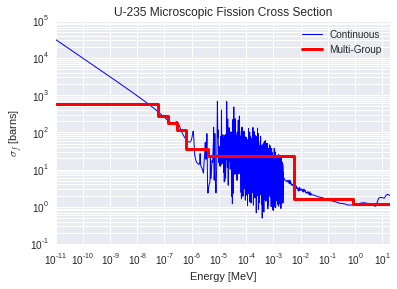
\includegraphics[width=0.8\linewidth]{figures/intro/u235-ce-mg-xs}
\caption[U-235 continuous energy and multi-group fission cross section]{U-235 continuous energy and 16-group fission cross section.}
\label{fig:chap1-u235-sigf}
\end{figure}

Many different engineering prescriptions have been developed to generate \ac{MGXS} for specific reactor configurations and spectra. In general, \ac{MGXS} generation schemes use a multi-level approach to decouple the energy, angular and spatial dimensions as depicted in Fig.~\ref{fig:chap1-multi-level-flow-chart}. The multi-level approach typically applies high-fidelity models of the energy self-shielding physics to low-fidelity geometric models of unique core components. The complexity of the energy treatment is then reduced at each level as larger and more complex geometric models are considered.

\begin{figure}
\centering
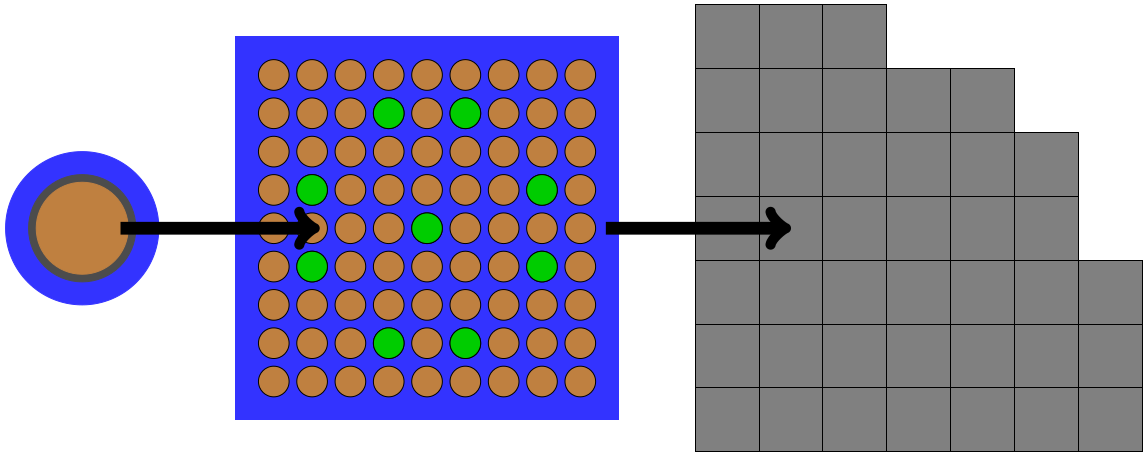
\includegraphics[width=0.9\linewidth]{figures/intro/multi-step-flow-chart}
\caption[Multi-level approach to reactor analysis]{Current multi-level framework for reactor analysis.}
\label{fig:chap1-multi-level-flow-chart}
\end{figure}

For example, the first stage for \ac{LWR} \ac{MGXS} generation attempts to capture energy self-shielding effects within simplified geometric models such as infinite fuel pin cells. This step typically condenses continuous energy cross sections to $\mathcal{O}(100)$ groups. These \ac{MGXS} are then used in a heterogeneous lattice physics calculation of an individual fuel assembly within an infinite lattice. The lattice physics calculation models spatial self-shielding effects between pins of various material compositions and condenses the \ac{MGXS} to a coarse energy structure of $\mathcal{O}(10)$ groups. In addition, the \ac{MGXS} may be spatially-homogenized across the entire fuel assembly or across each fuel pin within each assembly. Finally, the spatially-homogenized coarse \ac{MGXS} for each fuel assembly are used in a whole-core calculation composed of many fuel assemblies.

The multi-level approach uses a combination of models of varying complexity to optimize overall simulation speed with accuracy. However, this is typically done at the expense of generality. For example, some prior knowledge of the neutron energy spectra is required to design approximations to the flux for a particular reactor configuration. Furthermore, multi-level \ac{MGXS} generation schemes do not generally model inter-assembly physics or the effect of reflectors and other core heterogeneities on the spatial distribution of the flux. Instead, geometric heuristics are often used to embed spatial self-shielding effects in \ac{MGXS} for similarly shielded spatial zones (\textit{e.g.}, fuel pins with similar neighboring pins). The approximations to the energy and spatial variation of the flux introduce approximation error in whole-core calculations and limit the core design parameter space for which multi-level schemes may be applied. New reactor agnostic \ac{MGXS} generation methods are needed to enable deterministic transport-based methods to be as accurate and flexible as Monte Carlo in whole-core calculations.

%For reactors with a greater degree of spectral coupling, however, these approximations are not valid, resulting in ever larger datasets for the cross section generation process.

This thesis investigates the use of Monte Carlo methods to generate \ac{MGXS} for whole-core deterministic reactor analysis. Monte Carlo presents a natural approach to replace engineering prescriptions to approximate the flux with a stochastic approximation of the exact flux. The advantage of a \ac{MC}-based approach is that all of the relevant physics modeled in \ac{MC} may be directly embedded into \ac{MGXS}. This improvement in accuracy comes at the computational expense of converging group constant tallies to acceptably low uncertainties. \ac{MC} methods have increasingly been used to generate few group constants for coarse mesh diffusion, most notably by the Serpent \ac{MC} code~\cite{serpent2013manual}. However, there exist few rigorous and comprehensive analyses of \ac{MGXS} generation for heterogeneous fine mesh deterministic transport methods.

\begin{emphbox}
\textbf{This thesis develops and evaluates \ac{MC}-based methods to generate \ac{MGXS} for fine mesh deterministic neutron transport codes.}
\end{emphbox}

\vspace{-0.1in}

In addition, \ac{MC}-based \ac{MGXS} generation methods to date have retained the multi-level geometric framework to tabulate \ac{MGXS} for individual reactor components -- such as infinite fuel pins and/or assemblies -- for subsequent use in whole-core multi-group calculations. Although the use of \ac{MC} within a multi-level scheme eliminates the need to approximate the flux in energy, it does not account for spatial self-shielding effects throughout a reactor core. This thesis abandons the multi-level framework in place of a whole-core \ac{MC} calculation which simultaneously accounts for all energy and spatial self-shielding effects in a single step.

In theory, whole-core \ac{MC} calculations can be used to tally \ac{MGXS} in each spatial zone (\textit{e.g.}, 100 axial depletion zones within each of 50,000+ fuel pins in a \ac{PWR} core) to account for the spatial variation of the flux. However, such simulations have not been employed for practical reasons -- in particular, the large memory footprint and computational expense of performing such calculations has been prohibitive for \ac{MC} codes until recent years. Furthermore, roughly the same number of particle histories would be required to converge the \ac{MGXS} tallies in each spatial zone as would be required for a direct whole-core calculation by \ac{MC}. Hence, it would be more sensible to simply use \ac{MC} to compute the solution to the whole-core eigenvalue problem directly rather than use it to fully embed spatial self-shielding effects in \ac{MGXS} for deterministic transport codes. Therefore, in order for \ac{MC} to be practical for reactor agnostic fine mesh \ac{MGXS} generation, a new method is required to accelerate the convergence rate of the \ac{MGXS} tallies in each fine mesh region to a degree that is not possible for conventional whole-core Monte Carlo simulations. 

This thesis proposes to use statistical clustering methods to accelerate the convergence rate of whole-core \ac{MC} calculations for \ac{MGXS} generation. This novel approach relies on the fact that many distinct spatial zones across a reactor core experience similar if not identical spatial self-shielding effects, and therefore have similar if not identical \ac{MGXS}. The stochastic nature of \ac{MC} simulations will contribute statistical ``noise'' to the tally estimates for the \ac{MGXS}. As a result, the \ac{MGXS} estimates for similarly self-shielded spatial zones will form clusters which will converge as more particle histories are simulated. The goal of this thesis is to develop and apply algorithms to identify \ac{MGXS} clusters from ``noisy'' Monte Carlo tally data and to predict the true mean of each cluster prior to convergence. This methodology aims to generate \ac{MGXS} for deterministic neutron transport codes in a reactor agnostic and computationally efficient manner.

%The true mean of each cluster will then be used as the predicted estimate for the multi-group cross-section for each fine-mesh region in each cluster.

\begin{emphbox}
\textbf{This thesis uses statistical clustering algorithms to accelerate whole-core \ac{MC} calculations
which simultaneously model all energy and spatial self-shielding effects for fine mesh \ac{MGXS} generation in a single step.}
\end{emphbox}


%%%%%%%%%%%%%%%%%%%%%%%%%%%%%%%%%%%%%%%%%%%%%%%%%%%%%%%%%%%%%%%%%%%%%%%%%%%%%%%
\section{Thesis Objectives}
\label{sec:chap1-objectives}

The subject matter of this thesis is organized along two main themes:

\begin{itemize}
\item \textbf{\textit{Approximation Error}} -- Quantify and diagnose approximation error in \ac{MGXS} generated from \ac{MC} methods for simple heterogeneous benchmark problems.
\item \textbf{\textit{Statistical Clustering}} -- Develop statistical clustering methods to accelerate the convergence rate of \ac{MGXS} on heterogeneous \ac{MC} tally meshes.
\end{itemize}

The first theme of this thesis rigorously assesses the efficacy of \ac{MGXS} generation with \ac{MC} for fine mesh transport calculations. Some of the approximations made by \ac{MC}-based \ac{MGXS} generation are quantified, including the energy and spatial dependence of condensed \ac{MGXS}. An in-depth analysis of systematic bias resulting from constant-in-angle total \ac{MGXS} is presented, along with a scheme based on \ac{SPH} factors to compensate for this loss in accuracy. 

The second theme of this thesis develops a new methodology to simultaneously capture local and global spatial self-shielding effects in \ac{MGXS} for whole-core calculations. This scheme applies statistical clustering methods to accelerate the convergence rate of \ac{MGXS} tallied on fine, heterogeneous spatial meshes in Monte Carlo. The latent variable model which inspires the clustering paradigm is presented, along with a discussion of the implementation of a data pipeline to evaluate clustering algorithms for \ac{MGXS} generation. A series of increasingly complex heterogeneous benchmarks are modeled to empirically compare the accuracy and convergence rate of the approach with more traditional multi-level schemes for \ac{MC}-based MGXS generation.


%%%%%%%%%%%%%%%%%%%%%%%%%%%%%%%%%%%%%%%%%%%%%%%%%%%%%%%%%%%%%%%%%%%%%%%%%%%%%%%
\section{Thesis Outline}
\label{sec:chap1-outline}

This thesis is segmented into five Parts. Part I is comprised of this introductory chapter.

Part II discusses the relevant background information for this thesis. Chap.~\ref{chap:mgxs} reviews multi-group neutron transport theory and considers some common approximations made in \ac{MGXS} generation and multi-group transport codes. Chap.~\ref{chap:mgxs-mc} introduces Monte Carlo as an approach to generate \ac{MGXS}, and highlights relevant studies in the literature which have used \ac{MC} to generate \ac{MGXS}. Chap.~\ref{chap:workflow} presents the simulation workflow developed for this thesis to evaluate \ac{MC} for \ac{MGXS} generation, including the OpenMC, OpenMOC and OpenCG codes.

Part III diagnoses common sources of approximation error in \ac{MGXS} generation and multi-group transport methods. Chap. \ref{chap:biases} quantifies the impact of multi-group approximation error for simple, heterogeneous \ac{PWR} geometries. Chap.~\ref{chap:sph} presents an algorithmic approach to mitigate systematic biases resulting from constant-in-angle total \ac{MGXS} using \ac{SPH} factors, and motivates the need for future work to address this issue.

Part IV develops a novel approach based on statistical clustering methods to accelerate whole-core \ac{MC} calculations for \ac{MGXS} generation. Chap.~\ref{chap:benchmarks} analyzes the convergence rate of \ac{MGXS} datasets computed on fine spatial \ac{MC} tally meshes for a series of heterogeneous \ac{PWR} benchmark models to motivate this new methodology. Chap.~\ref{chap:quantify} quantifies the impact of using \ac{MGXS} which reflect inter-pin and inter-assembly spatial self-shielding effects on the solutions computed by multi-group deterministic transport methods. Chap.~\ref{chap:spatial} analyzes the emergence of \ac{MGXS} clusters due to spatial self-shielding with a variety of visual aids. Chap.~\ref{chap:unsupervised} outlines a latent variable model for clustering \ac{MGXS}, along with a data pipeline for unsupervised clustering to accelerate the \ac{MGXS} convergence rate. Chapter~\ref{chap:results} evaluates the impact of clustered \ac{MGXS} on the accuracy and convergence rate of the eigenvalue solutions computed by deterministic transport methods.

Part V is composed of Chapter~\ref{chap:conclusions} which summarizes the progress made in this thesis to chart a path forward for \ac{MC}-based \ac{MGXS} generation for whole-core deterministic transport methods.

%\begin{figure}
%\begin{subfigure}{\textwidth}
%  \centering
%  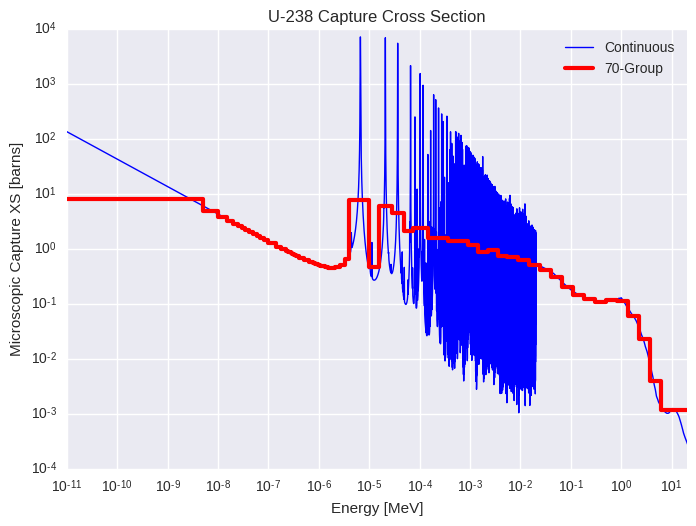
\includegraphics[width=0.9\linewidth]{figures/intro/u238-capture-70}
%  \caption{}
%\end{subfigure}
%\begin{subfigure}{\textwidth}
%  \centering
%  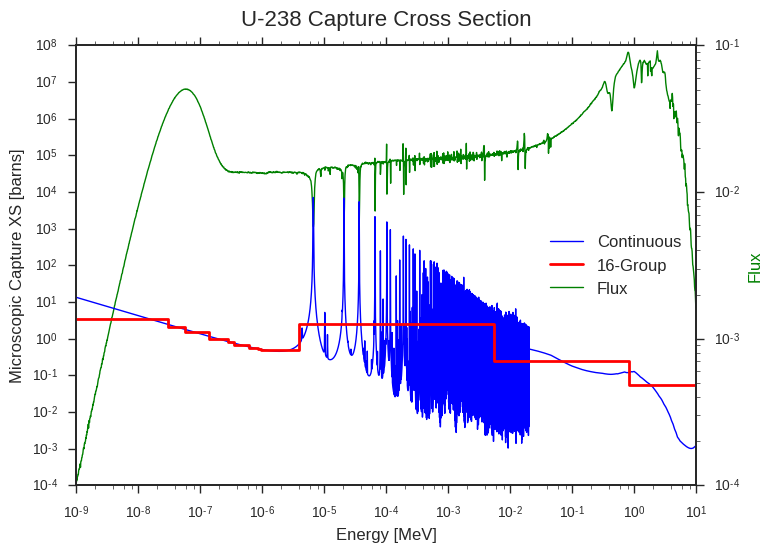
\includegraphics[width=0.9\linewidth]{figures/intro/u238-capture-16}
%  \caption{}
%\end{subfigure}
%\caption[Uranium-238 capture cross section]{Continuous energy and multi-group cross sections for U-238 capture in a PWR spectrum for 70-groups (a) and 16-groups (b).}
%\label{fig:pwr-ce-mg-xs}
%\end{figure}

